\documentclass[]{article}
\usepackage[top=2cm,bottom=2cm,left=2.5cm,right=2cm]{geometry}
\usepackage{amssymb}
\usepackage{amsmath}
\usepackage{tikz}

%opening
\title{$\epsilon$-NFA and Regex Equivalence In Lean}
\author{Eyal Barnea, Harry Cohen, Noam Jacobi}
\date{Winter 25-26 - Spring 26}
\begin{document}
%\verb|https://github.com/eyal3741/Formal-Matka/|
\maketitle
\begin{abstract}
	This project (\verb|https://github.com/eyal3741/Formal-Matka/|) proves the equivalence of the computational models $\epsilon$-NFA and regular expressions, as seen in Introduction To Set Theory And Automata ($02340129$), using the Lean proof assistant. During this project we have uncovered a gap between the definitions of the different types of Finite Automata and updated the definition of $\epsilon$-NFA to be on par with the definitions of both DFA and NFA.
\end{abstract}
\section{Overview Of Subject And Proof Idea}
As "We all remember the material of Introduction To Set Theory And Automata, since it is engraved on the tablet of our hearts"\footnote{Dr. Sarai Sheinvald, Logic For CS, Lecture 1}, it is known that the computational models of Deterministic Finite Automata (DFA), Non-Deterministic Finite Automata (NFA) and Non-Deterministic Finite Automata with $\epsilon$ transitions ($\epsilon$-NFA) are proven to have the same expressive power.In order to show their equivalence to Regular Expressions (Regex), we would need to show that for every $\epsilon$-NFA $A$, there exists a Regex $r$ such that $L(A)=L(r)$, and vice versa.\\
These two proofs (written in short below) turn out to be quite challenging in Lean, as Lean has many tools to and lemmas to prove problems in regard to mathematical problems, while for both Regex an automata "their underlying mathematical foundation is extremely poor (in that there is no rich theory underneath them, such as calculus, probability theory, group theory, etc.), and yet they give rise to very intricate problems. Since there are not many mathematical foundations to use, all we can use is our brain. Hence – fun!"\footnote{Assoc. Prof. Shaull Almagor, Automata Logic And Games, Lecture 1}
\subsection{$\forall r \exists A$:}
Since Regex is defined using Structural Induction, the proof follows in the same way:
\begin{itemize}
	\item 
	base:
	\begin{itemize}
		\item 
		The Empty Language: An Automata with no states.
		\item 
		The Empty Word: An Automata with one state, both starting and accepting, and no transitions.
		
		\begin{center}
			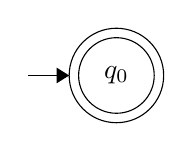
\begin{tikzpicture}[scale=0.2]
				\tikzstyle{every node}+=[inner sep=0pt]
				\draw [black] (25.5,-22.4) circle (3);
				\draw (25.5,-22.4) node {$q_0$};
				\draw [black] (25.5,-22.4) circle (2.4);
				\draw [black] (19.9,-22.4) -- (22.5,-22.4);
				\fill [black] (22.5,-22.4) -- (21.7,-21.9) -- (21.7,-22.9);
			\end{tikzpicture}
		\end{center}
		\item 
		A Single Character $\sigma$: An Automata with two state, one starting and the other accepting, and a single transition from the starting state to the accepting state using $\sigma$.
		\begin{center}
			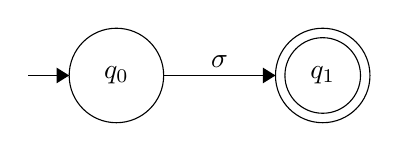
\begin{tikzpicture}[scale=0.2]
				\tikzstyle{every node}+=[inner sep=0pt]
				\draw [black] (25.5,-22.4) circle (3);
				\draw (25.5,-22.4) node {$q_0$};
				\draw [black] (38.6,-22.4) circle (3);
				\draw (38.6,-22.4) node {$q_1$};
				\draw [black] (38.6,-22.4) circle (2.4);
				\draw [black] (19.9,-22.4) -- (22.5,-22.4);
				\fill [black] (22.5,-22.4) -- (21.7,-21.9) -- (21.7,-22.9);
				\draw [black] (28.5,-22.4) -- (35.6,-22.4);
				\fill [black] (35.6,-22.4) -- (34.8,-21.9) -- (34.8,-22.9);
				\draw (32.05,-21.9) node [above] {$\sigma$};
			\end{tikzpicture}
		\end{center}
	\end{itemize}
	\item 
	step:
	\begin{itemize}
		\item
		The $+$ Operator: putting the two automata "side by side"
		\begin{center}
			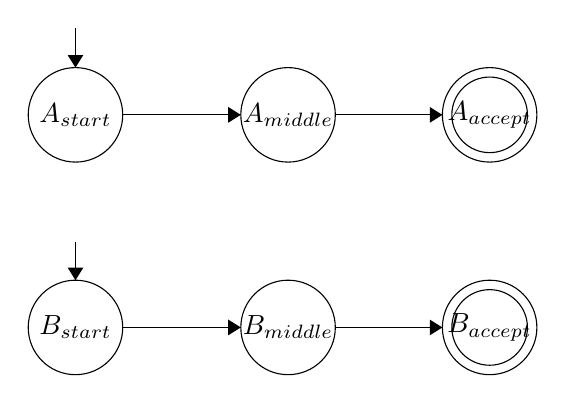
\begin{tikzpicture}[scale=0.2]
				\tikzstyle{every node}+=[inner sep=0pt]
				\draw [black] (15,-20.4) circle (3);
				\draw (15,-20.4) node {$A_{start}$};
				\draw [black] (28.5,-20.4) circle (3);
				\draw (28.5,-20.4) node {$A_{middle}$};
				\draw [black] (41.3,-20.4) circle (3);
				\draw (41.3,-20.4) node {$A_{accept}$};
				\draw [black] (41.3,-20.4) circle (2.4);
				\draw [black] (15,-33.9) circle (3);
				\draw (15,-33.9) node {$B_{start}$};
				\draw [black] (28.5,-33.9) circle (3);
				\draw (28.5,-33.9) node {$B_{middle}$};
				\draw [black] (41.3,-33.9) circle (3);
				\draw (41.3,-33.9) node {$B_{accept}$};
				\draw [black] (41.3,-33.9) circle (2.4);
				\draw [black] (18,-20.4) -- (25.5,-20.4);
				\fill [black] (25.5,-20.4) -- (24.7,-19.9) -- (24.7,-20.9);
				\draw [black] (31.5,-20.4) -- (38.3,-20.4);
				\fill [black] (38.3,-20.4) -- (37.5,-19.9) -- (37.5,-20.9);
				\draw [black] (18,-33.9) -- (25.5,-33.9);
				\fill [black] (25.5,-33.9) -- (24.7,-33.4) -- (24.7,-34.4);
				\draw [black] (31.5,-33.9) -- (38.3,-33.9);
				\fill [black] (38.3,-33.9) -- (37.5,-33.4) -- (37.5,-34.4);
				\draw [black] (15,-14.9) -- (15,-17.4);
				\fill [black] (15,-17.4) -- (15.5,-16.6) -- (14.5,-16.6);
				\draw [black] (15,-28.5) -- (15,-30.9);
				\fill [black] (15,-30.9) -- (15.5,-30.1) -- (14.5,-30.1);
			\end{tikzpicture}
		\end{center}
		
		\item 
		The $\cdot$ Operator: connecting the first automata's accepting states with an $\epsilon$ transition to the second's starting states
		\begin{center}
			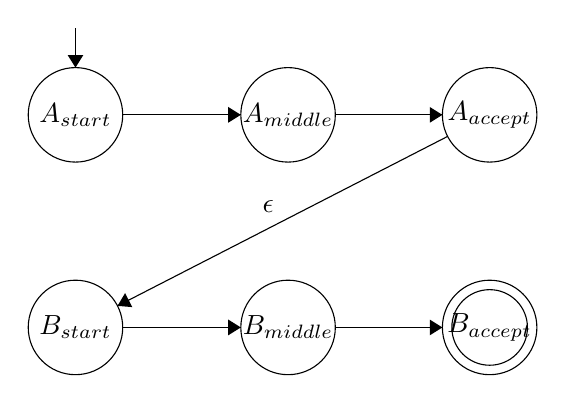
\begin{tikzpicture}[scale=0.2]
				\tikzstyle{every node}+=[inner sep=0pt]
				\draw [black] (15,-20.4) circle (3);
				\draw (15,-20.4) node {$A_{start}$};
				\draw [black] (28.5,-20.4) circle (3);
				\draw (28.5,-20.4) node {$A_{middle}$};
				\draw [black] (41.3,-20.4) circle (3);
				\draw (41.3,-20.4) node {$A_{accept}$};
				\draw [black] (15,-33.9) circle (3);
				\draw (15,-33.9) node {$B_{start}$};
				\draw [black] (28.5,-33.9) circle (3);
				\draw (28.5,-33.9) node {$B_{middle}$};
				\draw [black] (41.3,-33.9) circle (3);
				\draw (41.3,-33.9) node {$B_{accept}$};
				\draw [black] (41.3,-33.9) circle (2.4);
				\draw [black] (18,-20.4) -- (25.5,-20.4);
				\fill [black] (25.5,-20.4) -- (24.7,-19.9) -- (24.7,-20.9);
				\draw [black] (31.5,-20.4) -- (38.3,-20.4);
				\fill [black] (38.3,-20.4) -- (37.5,-19.9) -- (37.5,-20.9);
				\draw [black] (18,-33.9) -- (25.5,-33.9);
				\fill [black] (25.5,-33.9) -- (24.7,-33.4) -- (24.7,-34.4);
				\draw [black] (31.5,-33.9) -- (38.3,-33.9);
				\fill [black] (38.3,-33.9) -- (37.5,-33.4) -- (37.5,-34.4);
				\draw [black] (15,-14.9) -- (15,-17.4);
				\fill [black] (15,-17.4) -- (15.5,-16.6) -- (14.5,-16.6);
				\draw [black] (38.63,-21.77) -- (17.67,-32.53);
				\fill [black] (17.67,-32.53) -- (18.61,-32.61) -- (18.15,-31.72);
				\draw (27.24,-26.65) node [above] {$\epsilon$};
			\end{tikzpicture}
		\end{center}
		\item 
		The $*$ Operator: creating a singular starting and accepting state, connecting it with automata's starting states and the automata's accepting states to it with an $\epsilon$ transition
		\begin{center}
			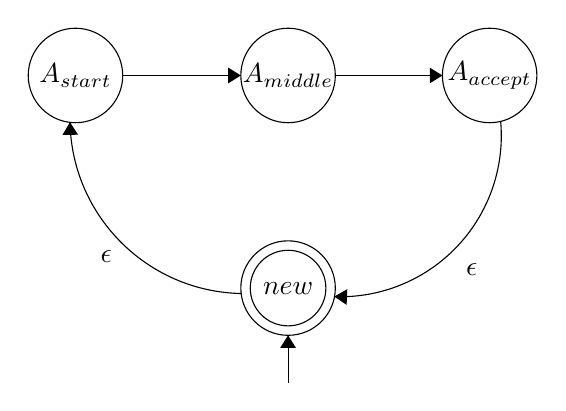
\begin{tikzpicture}[scale=0.2]
				\tikzstyle{every node}+=[inner sep=0pt]
				\draw [black] (15,-20.4) circle (3);
				\draw (15,-20.4) node {$A_{start}$};
				\draw [black] (28.5,-20.4) circle (3);
				\draw (28.5,-20.4) node {$A_{middle}$};
				\draw [black] (41.3,-20.4) circle (3);
				\draw (41.3,-20.4) node {$A_{accept}$};
				\draw [black] (28.5,-33.9) circle (3);
				\draw (28.5,-33.9) node {$new$};
				\draw [black] (28.5,-33.9) circle (2.4);
				\draw [black] (18,-20.4) -- (25.5,-20.4);
				\fill [black] (25.5,-20.4) -- (24.7,-19.9) -- (24.7,-20.9);
				\draw [black] (31.5,-20.4) -- (38.3,-20.4);
				\fill [black] (38.3,-20.4) -- (37.5,-19.9) -- (37.5,-20.9);
				\draw [black] (28.5,-39.9) -- (28.5,-36.9);
				\fill [black] (28.5,-36.9) -- (28,-37.7) -- (29,-37.7);
				\draw [black] (42,-23.306) arc (5.13888:-92.08964:10.229);
				\fill [black] (31.44,-34.44) -- (32.22,-34.97) -- (32.26,-33.97);
				\draw (39.77,-32.73) node [right] {$\epsilon$};
				\draw [black] (25.529,-34.246) arc (-91.10022:-178.89978:11.091);
				\fill [black] (14.65,-23.37) -- (14.17,-24.18) -- (15.17,-24.16);
				\draw (16.96,-31.48) node [below] {$\epsilon$};
			\end{tikzpicture}
		\end{center}
	\end{itemize}
\end{itemize}
\subsection{$\forall A \exists r$:}
We use Dynamic Programming to build a Regex describing all paths between any two states:
\begin{itemize}
	\item 
	base: the paths between two states $i,j$ without going through any state in the middle are the transitions  between them (or the empy word, if they are the same):
	$$r(i,j,0) = \sum_{\sigma \in \Sigma: \delta(i, \sigma) = j} \sigma + \begin{cases}
		\epsilon & i = j \,\text{or}\, \delta(i, \epsilon) = j\\
		&else
	\end{cases}$$
	\item 
	step: the paths between two states $i,j$ going through only states between $1...k$ are either
	\begin{itemize}
		\item 
		not going through $k$, thus going through only $1...k-1$
		\item 
		going through $k$, thus can be divided into the first time going to $k$ in the first time, going any number of times to $k$ again then finally going to $j$
	\end{itemize}
	$$r(i,j,k) = r(i,j,k-1) + r(i,k,k-1) \cdot r(k,k,k-1)^* \cdot r(k,j,k-1)$$
\end{itemize}
\section{Hardships Encountered}
\subsection{$\forall r \exists A$:}
\subsubsection{Working With Automata}
In lean automata, $\epsilon$-NFA are defined over a universe of states (and for the automata to be well defined, it is the responsibility of the user to make sure they use a finite set. seeing this, for ease of usage we chose to work over a universe of $\mathbb{N}$), where the reachable states are implicitly defined by the transition function, and any reference to a path within them is only in the form of the proposition "the word $x$ is a path between the states $i$ and $j$". In addition, said universe of states is not defined as finite. Thus, the following hardships emerge:
\begin{itemize}
	\item 
	If two automata share the name of some of their states, there is a need to rename them before using the automata together in any construction. Additionally, since the states of each automata are implicitly defined and may or may not be finite, the renaming must not take into account the size of the state group.
	\item 
	Concrete paths do not exist, as no information on any path is available.
\end{itemize}
In order to deal with said problems, we did the following:
\begin{itemize}
	\item 
	We used the injective functions of $f_0(x) = 2x$ and $f_1(x) = 2x + 1$, where $Img(f_0) \cup Img(f_1) = \mathbb{N}$ and $Img(f_0) \cap Img(f_1) = \emptyset$, to rename the states back into the same universe without any collisions.
	\item 
	We construct the automata in such a way that by only using the propositions we can deduce the critical information about the path, skipping over any need for concrete paths.
\end{itemize}
\subsubsection{Automata Equivalence}
In order to prove the steps of the structural induction, the following tools needed to be developed:
\begin{itemize}
	\item 
	Renaming Equivalence: After using one of the renaming functions ($f_0,f_1$), the resulting automata accepts the same words as the original, and has the same paths.
	\item 
	Automata Containment: Let $A = \langle Q^A, Q_0^A, \Sigma, \delta^A, F^A \rangle,\; B = \langle Q^B, Q_0^B, \Sigma, \delta^B, F^B \rangle$.\\ if $B \subseteq A$ (i.e. $Q^B \subseteq Q^A,\; Q_0^B \subseteq Q_0^A,\; \delta^B \subseteq \delta^A$ as we consider the transition functions as groups of transitions $,\; F^B \subseteq F^A$), a path in $B$ implies the existence of the same path in $A$.
\end{itemize}
\subsubsection{Composition}
The main hardship involved in the composition was separating the accepted words of the new automata back into words accepted by the original automata. Noticing that the $\mod 2$ of the original automata in the new automata's construction and that the crossing points between the two and the transition points between the two is the first automata's accepting and starting states, in order to do so we needed the following sub-proofs:
\begin{itemize}
	\item
	In-automata $\mod 2$ consistency beside from the crossing point.
	\item 
	Irreversibility of changing sub-automata from first to second.
	\item 
	With starting state (in first sub-automata) and accepting state (in second sub-automata) locations in mind, determining the existence of a crossing point for every accepting word.
\end{itemize}
\subsubsection{Kleene Closure}
The main hardship involved in kleene closure was, like in the composition's case, separating the accepted word into accepting sub-words. The only sign of a new sub-word is derived by the singular added "new" state. in order to make use of it we needed to do the following:
\begin{itemize}
	\item 
	Rename the original Automata's states into even integers and keeping the "new" state, now named 1, as the only odd state.
	\item 
	Carefully follow the combinatorically astounding amount of different cases regarding $\epsilon$-transitions and their roles in the first and new automata to find the first accepting sub word.
	\item 
	Recursively apply the previously-outlined lemma to find the other sub-words.
\end{itemize}
\subsubsection{Additional Notable Lean Hardships}
\begin{itemize}
	\item 
	At first, defining the renaming functions by using the "match" tools seemed like the perfect match, but after disambiguating the function for use in the proof has been difficult and unintuitive we have switched to the "if/else" tools.
	\item 
	When using inductions, many assumptions that were correct only for the base were dragged along for the steps, making the induction harder to prove int the best cases and incorrect the common ones. In order to bypass this problem, we used every trick in the lean textbook, from generalizing, renaming propositions and even opening new environments using "have" and new lemmas to keep the assumptions sterile.
	\item 
	The kleene closure proofed to be technically challenging, requiring both many edge cases and even a recursively-defined lemma for the different sub-words, proven to be decreasing by word length and used to leverage the lemma (lovingly) nicknamed "lemma of absolute evil".
\end{itemize}
\subsection{$\forall A \exists r$:}
\subsubsection{Finding A Lean Fitting Proof}
After reviewing the material of Introduction To Set Theory And Automata, We have found a proof that was quite hand-wavy, in which states of the automata are being removed one by one, the transitions to and from them merging into Regular Expressions until only two states remain, one starting and one accepting, with one "transition" between them being the equivalent Regex to the entire automata. this proof requires us to go through the following steps:
\begin{itemize}
	\item 
	Define "Regex Automata", which read in each transition an unknown number of characters, accepted by the regex of the transition.
	\item 
	Prove any lemma already proven for other automata that will be needed for the rest of this direction.
	\item 
	Prove that $A_r$, created by copying $\epsilon$-NFA $A$ and changing every transition $\sigma$ to the regex $[\sigma]$, is equivalent to $A$.
	\item
	Prove that every step of state removal and transition merging result in an equivalent Regex Automata with a lesser number of states (which are, unless deviated from existing implementations of automata, implicitly defined).
\end{itemize}
Seeing that, and with the help of Dr. Sarai Sheinvald, we have found the dynamic programming proof (as seen above). this proof, however, was not free of problems: the entire proof relies of out ability to discern whether the path taken goes through the state $k$, without the ability to talk about concrete paths. As a bypass to the concrete path problem, we have tried to "trim" the automata, removing any transition that would lead to a state not in $1-k,j$ but after a great deal of work and effort in this direction we have found a counter example that show trimming cannot work - on the following automata (left), reach from $q_2$ to $q_2$ going only through $1-1$:
\begin{center}
	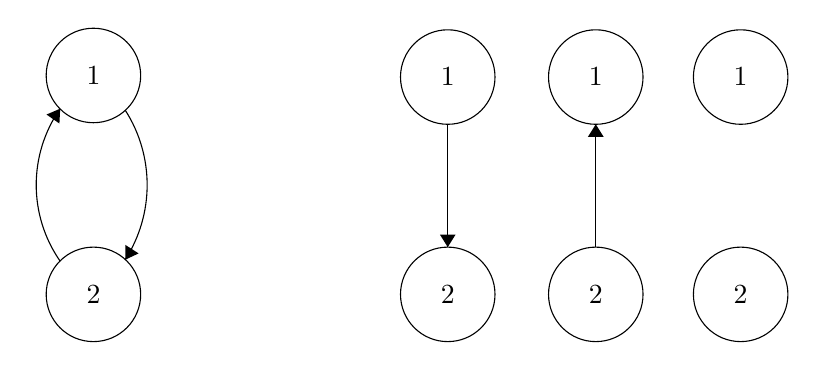
\begin{tikzpicture}[scale=0.2]
		\tikzstyle{every node}+=[inner sep=0pt]
		\draw [black] (16,-15.8) circle (3);
		\draw (16,-15.8) node {$1$};
		\draw [black] (16,-29.7) circle (3);
		\draw (16,-29.7) node {$2$};
		\draw [black] (38.5,-15.9) circle (3);
		\draw (38.5,-15.9) node {$1$};
		\draw [black] (47.9,-15.9) circle (3);
		\draw (47.9,-15.9) node {$1$};
		\draw [black] (57.1,-15.9) circle (3);
		\draw (57.1,-15.9) node {$1$};
		\draw [black] (38.5,-29.7) circle (3);
		\draw (38.5,-29.7) node {$2$};
		\draw [black] (47.9,-29.7) circle (3);
		\draw (47.9,-29.7) node {$2$};
		\draw [black] (57.1,-29.7) circle (3);
		\draw (57.1,-29.7) node {$2$};
		\draw [black] (13.888,-27.591) arc (-145.1147:-214.8853:8.465);
		\fill [black] (13.89,-17.91) -- (13.02,-18.28) -- (13.84,-18.85);
		\draw [black] (18.017,-18.001) arc (32.72403:-32.72403:8.785);
		\fill [black] (18.02,-27.5) -- (18.87,-27.1) -- (18.03,-26.56);
		\draw [black] (38.5,-18.9) -- (38.5,-26.7);
		\fill [black] (38.5,-26.7) -- (39,-25.9) -- (38,-25.9);
		\draw [black] (47.9,-26.7) -- (47.9,-18.9);
		\fill [black] (47.9,-18.9) -- (47.4,-19.7) -- (48.4,-19.7);
	\end{tikzpicture}
\end{center}
the only valid paths are $q_2$, $q_2-q_1-q_2$, but no way of trimming the automata (right) are able to produce only them.\\
Finally, after looking at the definitions of $DFA$ and $NFA$, we have discovered that concrete paths are defined in full and due to a mismatch in maintaining the definitions of all automata, $\epsilon$-NFA's definitions were not updated accordingly.
\subsubsection{Fixing The Gap In Lean Definition}
With the needed changes to Mathlib (\verb|https://github.com/leanprover-community/mathlib4/pull/40329|), many basic tools and lemmas needed to work with paths were still needing to be developed:
\begin{itemize}
	\item 
	Path Support: An ability to talk about the states visited in a given path.
	\item 
	Path Appending: Concatenation of two paths, one ending where the other begins, including definition, associativity, and support effects.
	\item 
	Path Containment: Identification of sub-paths, including definition, reflexivity and transitivity.
\end{itemize}
\subsubsection{Additional Notable Lean Hardships}
\begin{itemize}
	\item 
	The lean regex capabilities proved to be lacking, and as such we needed to define and prove some of the most basic tools - having a set of characters, creating a joint $+$ expression for them all and proving it functions as needed.
	\item 
	Defaultly, the types of the paths were defined by the transition labels, and so appending paths would cause problems since the different lists were identical in content, yet still not equal. in order to avoid this problem we have used both structures and the equality transport ($\blacktriangleright$) operator.
	\item 
	Path appending associativity was hard to prove in one of the directions, leading us after a thorough search to the usage of "grind" to solve that specific part.
\end{itemize}
\section{Lessons Learned and Recommendations}
\begin{itemize}
	\item 
	The scope of proofs is hard to determine and seemingly has no correlation to the depth of the material, but to the scope and ease of use of the existing tools in the field (and by proxy, to the popularity of the subject among the general lean user audience).
	\item 
	Correct division of proofs into lemmas helps both in keeping the proof readable and zeroing in on the hard part - while no proof has been trivial, many hours were saved by identifying the key tools needed.
	\item 
	Finding the documentation of the relevant mathlib files and identifying key lemmas leads to correct planning and fast proofs.
	\item 
	The course staff proved to be a powerful resource with vast knowledge, which were under-utilized during this project.
	\item 
	Considering the limitations of Lean while picking a proof changes significantly the "complexity" of the proof - what is easy for the human brain to understand might not be the best for lean to methodically proof. Making sure to write out every edge case helps to find the hidden assumptions and pinpoint ahead of time the hard parts.
\end{itemize}
\end{document}
